\providecommand{\main}{../../main}
\documentclass[../../main.tex]{subfiles}


\begin{document}

\chapter{Introduction to Deep Learning and Neural Networks}
\label{sec:NN_int}
\chaptermark{Neural Networks}
Machine learning has become widely used in many applications, one of them is the development of neural network based algorithm in the trigger system of some of the most advanced detectors active today, their aim is generally to discriminate the signal from the unwanted background.  
    
Deep learning methods, in particular, are often used and the Artificial Neural Networks are one of their key pillar, they are made of multiple layers from which the adjective ’deep’ derives. 
    
\section{Artificial Neural Networks}
\label{sec:ANN}
Nature has inspired many concepts that to us seem familiar in a variety of field, \acrfull{ann} is one of them that has taken as a model the animal brain. As for an biological brain in which many neurons are connected together though synapses, ANNs are computing systems made of a series of units, artificial neurons, connected among themselves.  
    
The simplest and the first architecture that we encounter is the \textit{perceptron}, that is used to describe an artificial neuron and is able to learn simple tasks. It was invented by Frank Rosenblatt in 1958 \cite{preceptron}. A perceptron takes as inputs a series of binary values $\bar{x}=\{x_1, \dots , x_n\}$ and gives as output a single binary value, mathematically this is a function $f(\bar{x},\varphi)$ where $\varphi$ is the set of parameters that defines our perceptron structure.  
    
These parameter set is composed by a vector of weights, a bias and a threshold ( $\text{w}_i,b, \delta \in \mathbb{R}$ )
    
\begin{equation}
    f(\bar{x},\varphi) = 
    \begin{cases}
    0\qquad\text{if}\quad\sum_{i=1}^N x_i \text{w}_i + b \leq \delta \\
    1\qquad\text{if}\quad\sum_{i=1}^N x_i \text{w}_i + b > \delta \\
    \end{cases}
\end{equation}

\begin{figure}[h]
    \centering
\includestandalone[height=6cm, width=\textwidth]{sections/03/Images/perceptron}
\caption{Internal structure of a perceptron.}
    \label{fig:perceptron}
\end{figure}
    
\section{Neural Networks architecture and key elements}
\label{sec:NN_arch}
\sectionmark{Key elements}
The perceptron is simple, but it is unable to solve complex tasks that Deep Learning field aim to tackle. In order to solve more complex tasks many of this structures are combined together giving birth to the so-called Artificial Neural Network. Such ANNs will be characterized by their architecture an type of substructure.  

In most common layout neurons are arranged in consecutive layers, each layer will receive the output of the previous one and will forward the result to the next, other operations can be performed in between. Layer are usually denoted as follows:
\begin{itemize}
    \item \textbf{Input layer}: the very first communication with the external world, its inputs are obviously given. An example could be a blurry image. 
    \item \textbf{Hidden layer}: Intermediate layer(s), they cannot be accessed form the outside.
    \item \textbf{Output layer}: Last layer, it will produce the prediction of the ANN, i.e. the cleaned image. 
\end{itemize}


A common procedure to mathematically describe a NN is move from the single neuron description to a per-layer description, doing so we can treat layers as single mathematical objects.  
It is clear that a layer has a set of inputs, some parameters and an output, which is the structure of a function. The description of the i-esim layer will be:  

\begin{equation}
    f_i(\bar{x_i}) = a_i\left(g_i(\bar{x_i}, \textbf{w}_i) + \bar{b_i} \right)
\end{equation}

We can distinguish many terms:
\begin{itemize}
    \item $\bar{x_i}$ : input vector;
    \item $\textbf{w}_i$ : matrix of free parameters, also called weights;
    \item $g_i()$ : operation between inputs and weights;
    \item $\bar{b_i}$ : bias vector, composed of free parameters;
    \item $a_i()$ : activation function computed to the result of layer operation, it plays a key role on the ability to solve or not the task assigned to the ANN;
\end{itemize}

Now it is possible to describe the full ANN in terms of collection of $N_L$ layers, its representation will be:

\begin{equation}
    \mathcal{F}_{N_L} = \left\{ f_N(\bar{x}), \textbf{w}, \bar{b}\right\}
\end{equation}

where $\textbf{w} = \{\textbf{w}_1 \dots \textbf{w}_{N_L}\}$ and 
$ \bar{b} = \{ \bar{b}_1 \dots  \bar{b}_{N_L}\}$ are respectively the set of all the layer weight and biases and the $f_N(\bar{x})$ is the composition of the $f_i(\bar{x_i})$
functions:
\begin{equation}
    f_N(\bar{x}) = f_{N_L} \circ f_{N_L-1}\circ\dots\circ f_2\circ f_1 (\bar{x}) 
\end{equation}

Now that an ANN is described the natural question is how to obtain free parameters $\textbf{w}$ and $\bar{b}$ optimal values. Starting from a particular ANN architecture and a given data set $\mathcal{D}$, it is possible to evaluate the free parameter though an iterative algorithm called \textit{training}. In this procedure a loss function is defined, the latter gives a score to the ANN current capability to solve the task, the training algorithm will try to minimize such values varying the free parameters.  

\subsection{Activation Functions}
\label{sec:NN_act}

As shown in the previous section an ANN layer can be mathematically represented as:  

\begin{equation}
    f_L^i (\bar{x_i})=a_i \left( \tilde{f}(\bar{x_i}, \textbf{w}_i) + \bar{b}_i \right) 
    \label{eq:layer_math}
\end{equation}

where $a_i$ is the so-called activation function. The choice of this function plays a crucial role in determining both the capability of the network of solving the assigned task and also  the time needed for it to be able to solve it efficiently, namely different activation function may need a longer training than others. The choice of this function depends on various factors but the most important ones surely are the position of the layer inside the network and the specific task it is trying to solve.

The position inside the network is relevant since the hidden layers of the network are usually built using activation functions with output values in $\mathbb{R}$ or $\mathbb{R}^+$ while, for the output layers, activation functions with values in $[0,1]$ or $[-1,1]$ are preferred, in order to interpret the results as a probability.
The specific task, on the other hand, mainly influences the activation function of the output layer since different tasks often requires a different output structure.
In the following a list of the most commonly used functions is presented.  

\begin{figure}[!h]
\begin{minipage}{0.45\textwidth}
    \centering
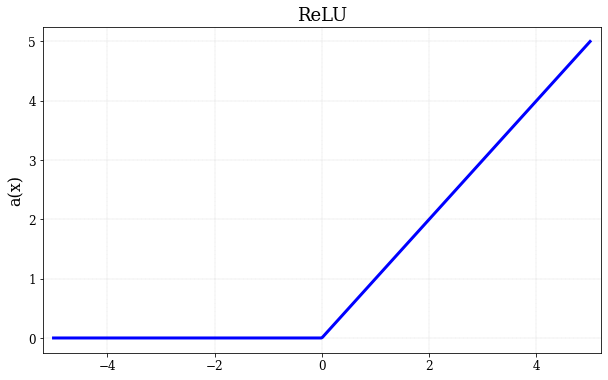
\includegraphics[width=\textwidth]{sections/03/Images/ReLU.png}
\caption{ReLU activation function}
    \label{fig:act_relu}
\end{minipage}
\hfill
\begin{minipage}{0.5\textwidth}
    \textbf{Rectified Linear Unit (ReLU)}
   \begin{align}
        a(x) &=
        \begin{cases}
        x   & \text{if } x > 0 \\
        0  & \text{if } x \leq 0 
  \end{cases}
\end{align}
The ReLU \cite{relu} is a continuous function with a point of non differentiability at 0. Despite being non differentiable - which is a point required for the back propagation step - this function is still implemented, mostly in the hidden layers of a network, due to its fast computation time. 
\end{minipage}
\end{figure}  


\begin{figure}[!h]

\begin{minipage}{0.5\textwidth}
    \textbf{Exponential Linear Unit (ELU)}
   \begin{align}
        a(x) &= 
        \begin{cases}
        \alpha \left(e^x -1\right)  & \text{if } x \leq 0 \\
        x  & \text{if } x > 0 
  \end{cases}
\end{align}
The ELU\cite{elu} activation functions is an improvement over the ReLU. In this case the negative values have an actual activation instead of being set to zero which may help the estimation of the network parameters. The drawback of choosing this function is an increase in the computational cost since an exponential operation is included. 
\end{minipage}
\hfill
\begin{minipage}{0.45\textwidth}
    \centering
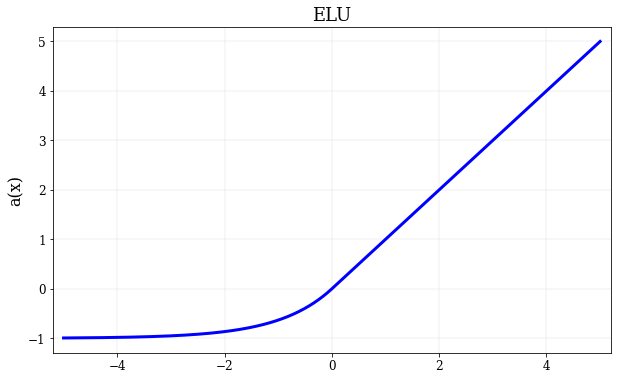
\includegraphics[width=\textwidth]{sections/03/Images/ELU.png}
\caption{ELU activation function}
    \label{fig:elu}
\end{minipage}
\end{figure}  


\begin{figure}[!h]
\begin{minipage}{0.45\textwidth}
    \centering
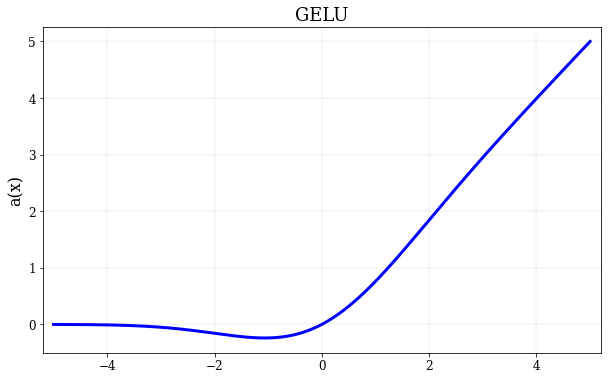
\includegraphics[width=\textwidth]{sections/03/Images/GELU.png}
\caption{GELU activation function}
    \label{fig:gelu}
\end{minipage}
\hfill
\begin{minipage}{0.5\textwidth}
    \textbf{Gaussian Error Linear Unit (GELU)}
   \begin{equation}
       a(x) = \frac{1}{2} x \left( 1+\text{erf} \left( \frac{x}{\sqrt{2}}\right)\right)
   \end{equation}
   The GELU\cite{gelu} is one of the newest activation functions. It was implemented in some of the most recent Deep Learining applications proving to be one of the best activations in the Natural Language Processing field\cite{bert,gpt}. 
\end{minipage}
\end{figure}  


\begin{figure}[!h]
\begin{minipage}{0.5\textwidth}
    \textbf{Binary step} or \textbf{Binary}
      \begin{align}
        a(x) &=
        \begin{cases}
        1   & \text{if } x \geq 0 \\
        -1  & \text{if } x < 0 
  \end{cases}
\end{align}
Neurons using this function are also called linear threshold units (LTU). This type of neurons can be used for solving simple tasks, but are not able to solve complex tasks like multiclass classifications. Often used in the so called Binarized Neural Networks (BNN).
\end{minipage}
\hfill
\begin{minipage}{0.45\textwidth}

    \centering
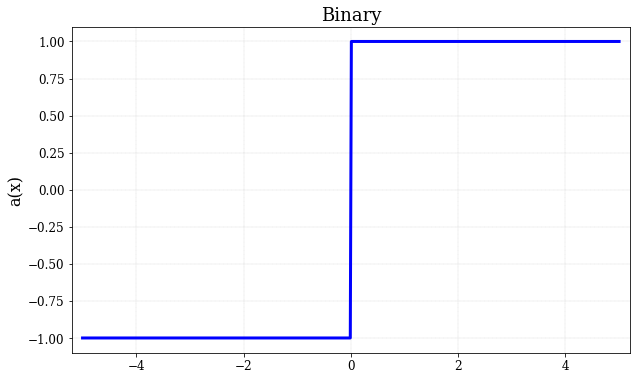
\includegraphics[width=\textwidth]{sections/03/Images/Binary.png}
\caption{Step activation function}
    \label{fig:act_step}
\end{minipage}
\end{figure}  


\begin{figure}[!h]
\begin{minipage}{0.45\textwidth}

    \centering
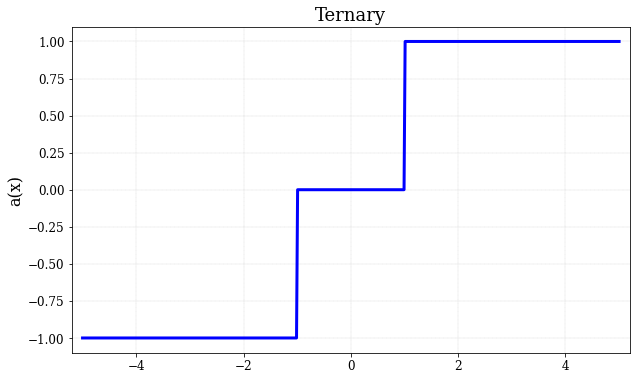
\includegraphics[width=\textwidth]{sections/03/Images/Ternary.png}
\caption{Ternary activation function}
    \label{fig:act_ter}
\end{minipage}
\hfill
\begin{minipage}{0.5\textwidth}
    \textbf{Ternary step} or \textbf{Ternary}
   \begin{align}
        a(x) &=
        \begin{cases}
        1   & \text{if } x \geq 1 \\
        0   & \text{if } -1 < x < 1 \\
        -1  & \text{if } x \leq -1
        \end{cases}
    \end{align}
   Quantized version of the hyperbolic tangent, employed mostly on the so-called Ternarized Neural Networks (TNN). Its usefulness lies on the fact that the operations can be mapped to trivial combinatorial ones. 
\end{minipage}
\end{figure}  


\begin{figure}[!h]

\begin{minipage}{0.5\textwidth}
    \textbf{Sigmoid} or \textbf{Soft step}
   \begin{equation}
       a(x) =\frac{1}{1+e^{-x}}
   \end{equation}
   The sigmoid function provides an output value in $[0,1]$ and it is differentiable in every point. This properties makes it one of the most used activation functions for the last layer of an ANN.
\end{minipage}
\hfill
\begin{minipage}{0.45\textwidth}

    \centering
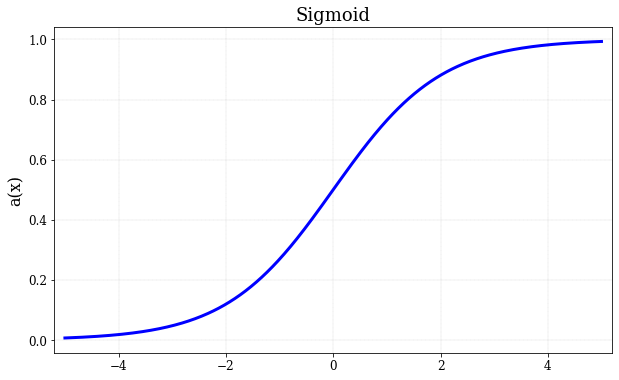
\includegraphics[width=\textwidth]{sections/03/Images/Sigmoid.png}
\caption{Sigmoid activation function}
    \label{fig:act_sig}
\end{minipage}
\end{figure}  


\begin{figure}[h!]
\begin{minipage}{0.45\textwidth}
    \centering
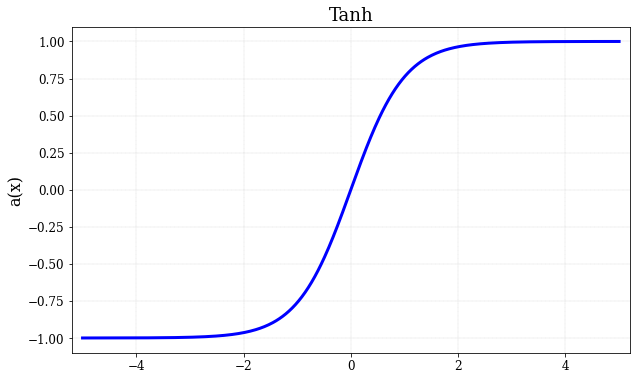
\includegraphics[width=\textwidth]{sections/03/Images/Tanh.png}
\caption{Hyperbolic tangent activation function}
    \label{fig:act_tanh}
\end{minipage}
\hfill
\begin{minipage}{0.5\textwidth}
    \textbf{Hyperbolic tangent}
   \begin{equation}
       a(x) =\frac{e^x-e^{-x}}{e^x+e^{-x}}
   \end{equation}
The hyperbolic tangent has similar properties to the sigmoid function. Its output is however in $[-1,1]$ which may speed up convergence in some applications.
\end{minipage}
\end{figure} 

\begin{figure}[h!]
\textbf{Softmax} \\

\begin{equation}
       a_i(\bold{x}) =\frac{e^{x_i}}{\sum_{j=1}^{K} e^{x_j}}
   \end{equation}
 
The softmax function takes as input a vector $\bold{x}$ of $K$ real numbers, and normalizes it into a probability distribution consisting of K probabilities proportional to the exponentials of the input numbers. After applying softmax, each component will be in the interval $\left(0,1\right)$ and the components will add up to 1, so that they can be interpreted as probabilities. Furthermore, the larger input components will correspond to larger probabilities. Generally used for multi-class classification.

\end{figure}

\vfill



\clearpage
    
\subsection{Dense Neural Network}
\label{sec:DNN}
Dense neural networks, DNNs in the following, are ANNs with a number of fully connected hidden layers. This leads to a large number of connection between the layers, from which the 'dense' adjective derives.  

Following directly from this denominations the fully connected layers that compose a Dense Neural Network are called Dense Layers. As it was mentioned in section \ref{sec:ANN}, a given layer is defined by the operation between inputs and weights; in this case this function is denoted with $f_D$, the mathematical representation is the dot product ($\cdot$).

\begin{equation}
    f_D (\bar{x})=a_i \left( \bar{x} \cdot \textbf{w} + \bar{b}_i \right) 
    \label{eq:layer_dense}
\end{equation}

Depending on the structure of the input vector $\bar{x}$ and on the weight tensor $\boldsymbol{w}$ the dot product represent a different mathematical operation, specifically:
\begin{itemize}
    \item if both $\bar{x}$ and $\textbf{w}$ are 1-dimensional vectors the dot product corresponds to the inner product of the two:
    \item if both $\bar{x}$ and $\textbf{w}$ are 2-dimensional, namely they are matrices, the dot product corresponds to the matrix-matrix multiplication of the two
     \item if either one is a scalar value then the dot product corresponds to a simple multiplication where the scalar is used as a factor
     \item if $\bar{x}$ and $\boldsymbol{w}$ respectively are an N-dimension and M-dimension tensor the dot product becomes a sum product over their last dimensions
\end{itemize}

\begin{figure}[h]
    \centering
    \includestandalone[width=0.8\textwidth]{sections/03/Images/DNN}
    \caption{Example of the structure of a Dense Neural Network. The neurons of each layer are represented by circles while the grey lines represent connections between them.}
    \label{fig:dnn_example}
\end{figure}

One of the main drawbacks of the usage of \acrshort{dnn}s, in particular on fast inference requirements, is however the number of free parameters. Dense layers are in fact characterized by an high number of weights and, due to the fully connected structure of the network, the total number of parameters grows fast with each additional layer. 
A too high number of parameters may lead to two main issues. The first problem one may encounter is the impossibility, during the training procedure, of correctly estimating the optimal network parameters. The second possible issue is the so-called over-fitting problem, namely the network adapts too well to the data on which it is trained with, but gives wrong predictions when tested on other datasets.  
%A brief explanation of this issue is discussed in \secref{fit_over_under}.
To avoid this issues the number of free parameters can be controlled, working on two factors:  shape of the input vector, which depends on the specific tasks and  number of neurons in each layer, which can be selected in order to reach the best compromise between performances and model complexity.
        
\subsection{Convolutional Neural Network}
\label{sec:CNN}

Another type on ANN is the so-called Convolutional Neural Network, also known as \acrshort{cnn}. As the name suggests the key mathematical operation in the layers of this type of network is the convolution. For this reason, this layers are called Convolutional Layers, from which the CNN name derives.

The key elements of a convolutional layers are the so-called filters. The output of a convolutional layer in fact computed as the resulting vector of the discrete convolution of the input values with each filter. 

\begin{wrapfigure}{l}{0.5\textwidth}
    \centering
    \includestandalone[width=0.5\textwidth]{sections/03/Images/CNN}
    \caption{Example of the combination of a convolutional layer with one 1 dimensional filter and a max pooling layer performing.  }
    \label{fig:cnn_tot}
    %\vspace{-1cm}
\end{wrapfigure}
The filters of a CNN have the same role of the weight tensor of a DNN and are in fact the free parameters of the network, whose optimization is performed during the training. In Fig. \ref{fig:cnn_filter} an example of the result of the application of a filter to a 2-dimensional input is shown.

In most of the common implementations however CNNs are not composed of only convolutional layers. They are in fact are made as an alternation of convolutional and pooling layers, where the latter is used to  perform a non-linear down-sampling on the output of a convolutional layer. 
More specifically a pooling layer divides its input in a series of regions called "pools" and applies a function to each one.
The resulting value from all pools is then combined and used as the output of the layer.
An example of the combination of these two layers is shown in \ref{fig:cnn_tot}.

Many choices for both the size of the pools and the function to apply are possible however one of the most common implementation is a max-pooling layer with a 2x2 pool size, namely a layer that divides the input in 2x2 regions and takes the highest value from each of them. A example of the application of this type of layer is shown in Fig. \ref{fig:cnn_pool}. 

\begin{figure}[h]
    \centering
    \includestandalone[width=\textwidth]{sections/03/Images/cnn_filter}
    \caption{Example of the application of a filter over a 2 dimensional input. The resulting matrix is computed as the discrete convolution of the input with the filter values.}
    \label{fig:cnn_filter}
\end{figure}

\begin{figure}[h]
    \centering
    \includestandalone[ width=0.78\textwidth]{sections/03/Images/cnn_pool} %0.78
    \caption{Example of the application of the max pooling operation over a 2 dimensional input, with 2x2 pool size. The resulting matrix is computed as the maximum value of each 2x2 pool.}
    \label{fig:cnn_pool}
\end{figure}


%\begin{wrapfigure}{r}{0.5\textwidth}
%    \centering
%  \includestandalone[height=7cm, width=0.6\textwidth]{images/networks/CNN}
%    \caption{cnn }
%    \label{fig:cnn_tot}
%\end{wrapfigure}
  
\section{Loss Functions}
\label{sec:NN_loss}

After the choice of the ANN type and its internal structure the next step is to choose the so-called loss function, also known as risk or cost function\cite{lossfunc}. The role of the loss function is to quantify how good the predicting power of the network is. Its choice plays a crucial role in the learning procedure.  

In most Deep Learning application the role of the learning algorithm is in fact to estimate the best set of parameters that are able to minimize the value of the loss function over a set of given input values. The choice of this function is therefore really important since it may greatly influence the final ability of the model of producing correct predictions.

As for the activation function many choices for the loss function are possible. In the following we present a brief list of the ones implemented in the most common applications:
\begin{itemize}
    \item \textbf{Mean Squared Error} or \textbf{L2 Loss}:\\
    This loss computes the average of the squared distance between the correct label associated to a sample, $y_{i,T}$ and the predicted one, $y_{i,P}$:
    \begin{equation}
        L_{MSE}= \frac{1}{N}\sum_{i=1}^N \left(y_{i,T}-y_{i,P}\right)^2
    \end{equation}
    This function is mostly implemented in regression tasks and is characterized by the heavy penalization imposed on predicted values very distant from their correct label. 
    \item \textbf{Mean Absolute Error} or \textbf{L1 Loss}:\\
    This loss computes the average of the absolute distance between the correct label associated to a sample, $y_{i,T}$ and the predicted one, $y_{i,P}$:
    \begin{equation}
        L_{MAE}= \frac{1}{N}\sum_{i=1}^N \left|y_{i,T}-y_{i,P}\right|
    \end{equation}
    Similarly to the L2 loss also the L1 is used in regression tasks but it penalizes more many small deviation from the correct label than few very distant ones. The main drawback of the L1 loss is the necessity of more complex tools for the computations of the gradient, with respect to the L2 loss, whose gradient can be easily computed exploiting its mathematical properties. 
\item \textbf{Hinge Loss}:\\
    The hinge loss is mostly famous for its implementation in Support Vector Machines (SVMs). As for the previous losses the Hinge one is a function of the true, $y_{i,T}$ and  predicted label, $y_{i,P}$ but with the constraint of them being either $\pm 1$:
    \begin{equation}
        L_{H}= \sum_{i=1}^N \max\left( 1-y_{i,T}*y_{i,P},0\right)
    \end{equation}
\item \textbf{Binary Cross Entropy Loss}:\\
    This function is the standard loss implemented for the binary classification tasks. It is computed using the true label associated to the i-th sample, requested to be a binary value, $y_{i,T}\in{0,1}$ and the probability $p_{i}$ of it being associated to the class indicated with $y_{T}=1$. With this notation the loss function is written as:
    \begin{equation}
        L_{BCE}= -\sum_{i=1}^N\left[ y_{i,T}\log(p_i)+
        \left(1- y_{i,T}\right)\log(1-p_i)\right]
    \end{equation}
    This loss function heavily penalizes confident but wrong predictions. 
\item \textbf{Categorical Cross Entropy Loss}:\\
    This loss function is the natural generalization of the previous one. As such it is the standard function implemented in multi-class classification tasks. Considering a classification tasks with $M>2$ classes, we can define: 
    \begin{equation}
        L_{CCE} = -\sum_{i=1}^N \sum_{c=1}^M  \left[
        y_{i,c}\log(p_{i,c}) + (1-y_{i,c})\log(1-p_{i,c})
        \right]
    \end{equation}
    where $p_{i,c}$, represent the predicted probability of the i-th belongin to the class $c$ and $y_{i,c}$ is a binary number equal to 1 only for the true class of the sample.
\item \textbf{Kullback-Leibler Divergence}:\\
   This loss function, commonly used in mathematical statistic as a difference measure between distribution, has proven its efficiency also for Deep Learning methods\cite{kullbackeff, kullbackeff2}. Indicating with $p_i$ and $q_i$ respectively the predicted and true label of a sample:
    \begin{equation}
        L_{KL} = - \left( \sum_{i=1}^{M} p_{i} \log{q_{i}} - \sum_{i=1}^{M} p_{i} \log{p_{i}} \right)
    \end{equation}
    
\end{itemize}
    
\section{Training workflow}
\label{sec:NN_training}

Training a model is in simple terms find minima of the loss function varying the layers hyper-parameters. This process involve multiple steps.

The data set must be divided in three different subsets:
\begin{itemize}
    \item The training set, the largest one, is used to teach the model its features.
    \item The validation set is used after each training epoch to check if the learning is proceeding in the right way.
    \item The test set is never used during the training step, it is used only after it to, as it name suggests, test the model. 
\end{itemize}

Once the data is split a loss function and an optimizer algorithm is selected.ADAM optimizer \cite{adam} is one of the most used, it belongs to the group of adaptive optimizers. This group instead of using a fixed learning rate adapt it to each parameters.
The power of this type of methods lies in its ability to adjust the amount of updates a specific parameter receives, based on both the importance and the frequency of the features connected to it.   

When adaptive learning methods, such as Adam, are not used as optimizers, it can be useful to do something that allows to modify the learning rate. It is indeed always better to have a large step-size at the beginning to guarantee a fast algorithm, but the learning rate should be further reduced in order to reach the global minimum without causing overshoot. An example is sketched in Fig.\ref{fig:learning rate}. 

\begin{figure}[h]
    \centering
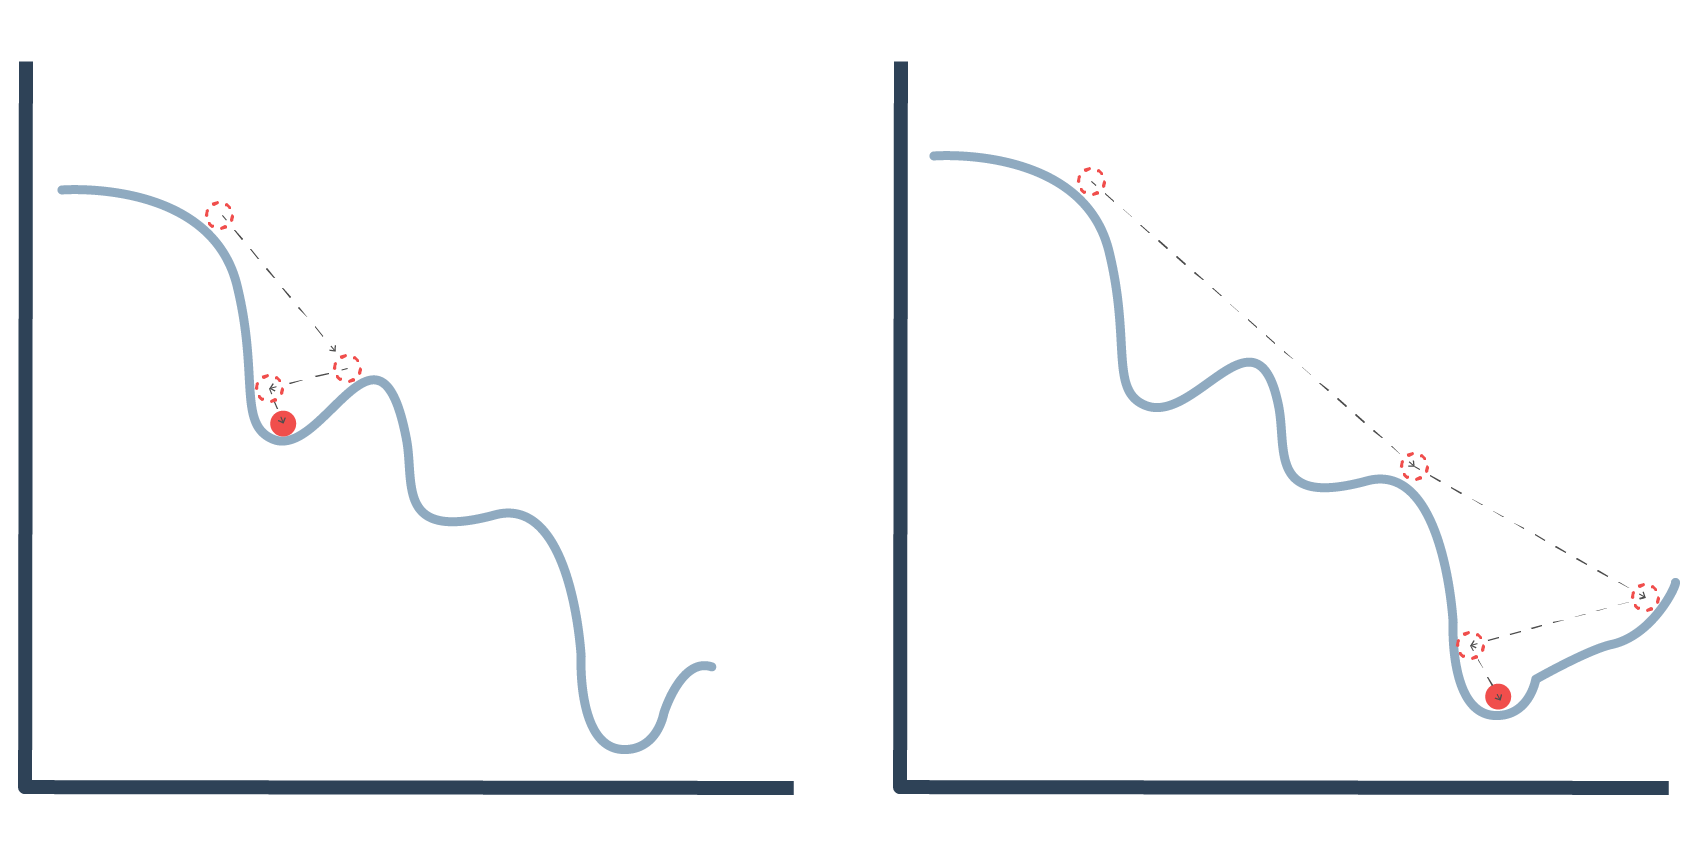
\includegraphics[width=0.75\textwidth]{sections/03/Images/Learning_rate.png}
\caption{Big steps are useful ate the beginning, smaller near the minimum}
    \label{fig:learning rate}
\end{figure}


\subsection{Regularization}\label{regularization}

Regularization is one of the central topics in the Machine Learning framework. Its goal is to reduce the generalized error, namely the error on a test set, while not modifying the error on the training set. The regularization topic is directly connected to the overfitting issue, which is the tendency of the model to fit too well the training set leaving aside its the general feature, regularization is in fact one of the most robust ways to prevent it.

The regularization is implemented defining a new regularized loss function, obtained by adding an additional term to the starting one. Indicating with $L(\boldsymbol{w},\bar{b})$ the loss function and its dependence on the weight and biases of the network, we define the regularized loss function $J(\mathbf{w}, \vec{b})$ as:
\begin{equation}
J(\mathbf{w}, \vec{b})=L(\mathbf{w}, \vec{b})+ \lambda\Omega(\mathbf{w})
\end{equation}

where $\lambda$ is a parameter that regulates the importance of the regularization respect to the loss and the $\Omega(\mathbf{w})$ is a function depending on the weights of the network. 


\begin{figure}[h]
    \centering
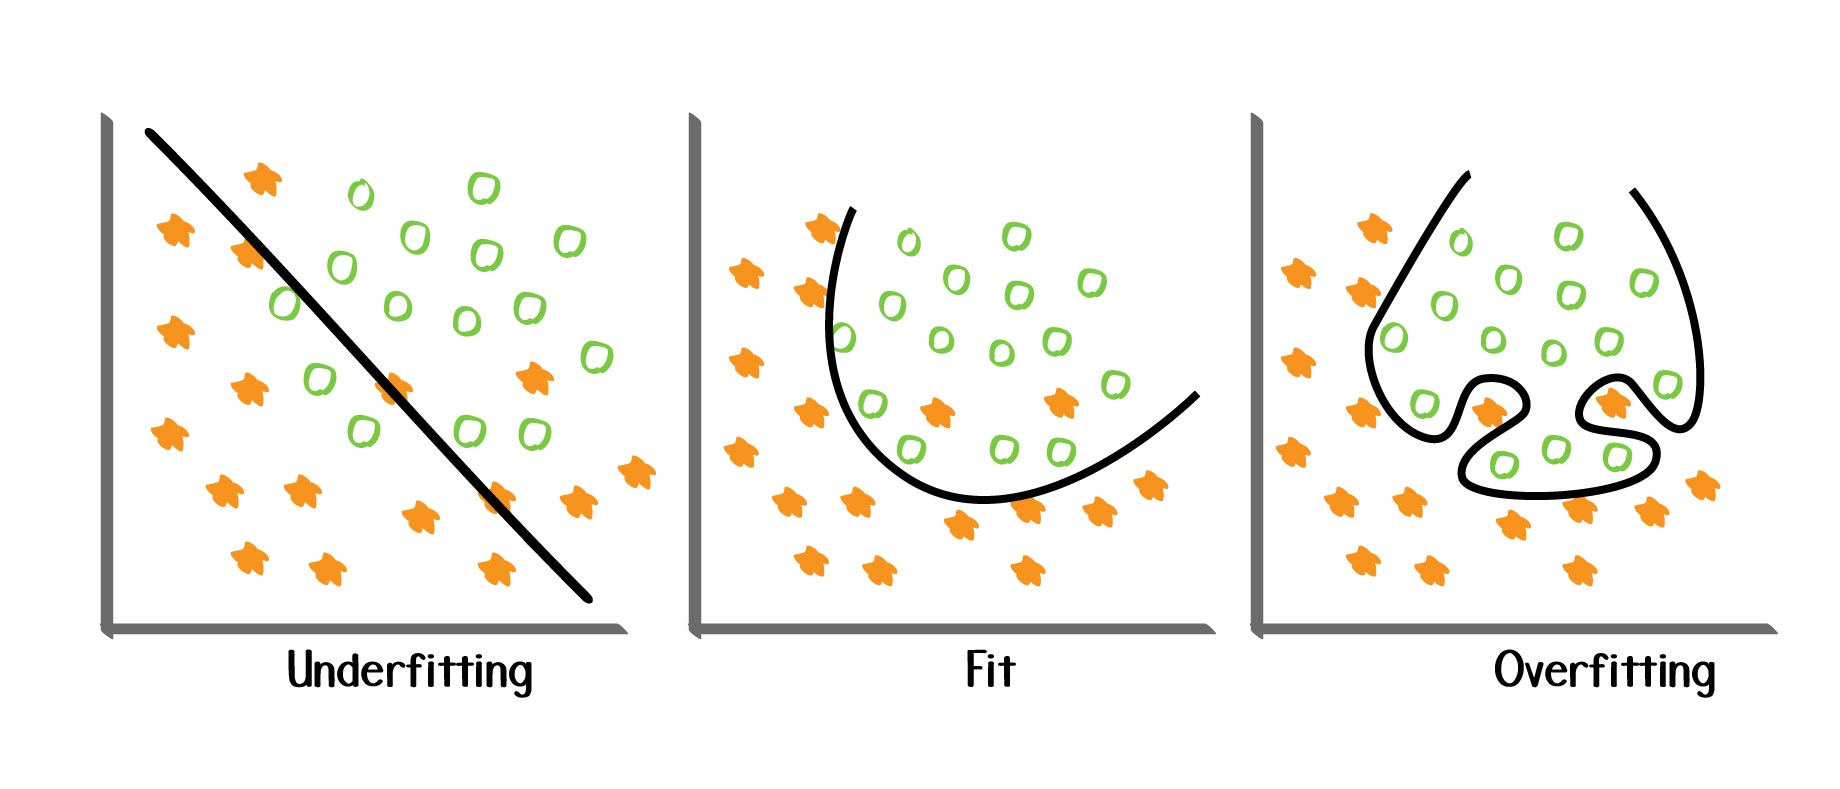
\includegraphics[width=0.85\textwidth]{sections/03/Images/ML_issues.jpg}
\caption{Overfitting and underfitting issues}
    \label{fig:overfitting}
\end{figure}

In most application the choice for the $\Omega(\mathbf{w})$ function is mainly restricted between to two alternatives:
\begin{itemize}
    \item \textbf{L1 regularization}: $\Omega_{L1}(\mathbf{w}) = \sum_{i=1}^N |\text{w}_i|$
    \item \textbf{L2 regularization}: $\Omega_{L2}(\mathbf{w}) = \sum_{i=1}^N \text{w}_i^2$
\end{itemize}

The main difference between the two is the macroscopic effect obtained after their implementation. The L1 regularization in fact tends to reduce the number of features that influences the final prediction while the L2 regularization reduces the influence that each feature has on it. The final choice between the two then depends on what the user wants to achieve but may also depend on the specific use case.
    
\end{document}